\documentclass[11pt,a4paper]{article}

% ---------- Packages ----------
\usepackage[margin=2.4cm]{geometry}
\usepackage[utf8]{inputenc}
\usepackage[T1]{fontenc}
\usepackage{booktabs}
\usepackage{longtable}
\usepackage{array}
\usepackage{tabularx}
\usepackage{enumitem}
\usepackage[hidelinks]{hyperref}
\usepackage{titlesec}
\usepackage{fancyhdr}
\usepackage{tikz}
\usepackage{float}
\usetikzlibrary{shapes.geometric, positioning, arrows.meta}

\setlist[itemize]{topsep=4pt, itemsep=4pt, parsep=0pt}
\setlist[enumerate]{topsep=4pt, itemsep=4pt, parsep=0pt}

\titleformat{\section}{\normalfont\Large\bfseries}{\thesection}{1em}{}
\titleformat{\subsection}{\normalfont\large\bfseries}{\thesubsection}{1em}{}
\titleformat{\subsubsection}{\normalfont\normalsize\bfseries}{\thesubsubsection}{1em}{}

\pagestyle{fancy}
\fancyhf{}
\renewcommand{\headrulewidth}{0.4pt}
\fancyhead[L]{\small Software Design Document -- VFMS}
\fancyhead[R]{\small\thepage}

\renewcommand{\arraystretch}{1.4}
\setlength{\tabcolsep}{8pt}

\begin{document}

% ==================== Cover Page ====================
\begin{titlepage}
\centering
\vspace*{2cm}
{\LARGE\bfseries Software Design Document}\\[0.5cm]
{\Large Vehicle Fleet Management System (VFMS)}\\[2cm]

\begin{tabular}{|p{5cm}|p{8cm}|}
\hline
Project Title & Vehicle Fleet Management System (VFMS) \\ \hline
Domain / Category & Vehicle Fleet Management System \\ \hline
Team Number & Team 10 \\ \hline
Member 1 & Tobo Mohlamonyane (47812036) \\ \hline
Member 2 & TJ Mnisi (51470470) \\ \hline
Member 3 & Karabo Makgala (50081659) \\ \hline

Submission Date & 13/09/2026 \\ \hline
SDD Version & v1.0 \\ \hline
Related SRS Version & v1.0 \\ \hline
\end{tabular}

\vspace{2cm}
Submitted in Partial Fulfilment of the Requirements of\\
Software Engineering Module (CMPG224)\\
North-West University, Mafikeng
\end{titlepage}

% ==================== Project Team ====================
\section*{Project Team and Approvals}

\begin{table}[H]
\centering
\begin{tabularx}{\textwidth}{|X|X|X|}
\hline
\textbf{Role} & \textbf{Name} & \textbf{Student Number} \\
\hline
Backend Developer & Tobo Mohlamonyane & 47812036 \\
\hline
Database Engineer & TJ Mnisi & 51470470 \\
\hline
Security \& DevOps Engineer / Backend Developer & Karabo Makgala & 50081659 \\
\hline
\multicolumn{3}{|c|}{\textbf{Client Representative}} \\
\hline
Lecturer / Client Representative & Prof. Bassey Isong &  \\
\hline
\end{tabularx}
\end{table}

\clearpage
\tableofcontents
\newpage

% ==================== 1. Introduction ====================
\section{Introduction}

\subsection{What This System Does}
The Vehicle Fleet Management System (VFMS) is a web application that helps a company keep track of its vehicles, drivers, and vehicle maintenance in one place. Many small companies currently manage this information using spreadsheets, which are easy to lose, hard to search through, and not secure. VFMS solves this by giving every vehicle and driver its own digital record, letting staff quickly find the information they need, and making sure only the right people can see sensitive details, such as a driver's licence number.

VFMS is being built to support six core features:
\begin{itemize}
    \item Adding and viewing vehicle details (registration number, model, year, status)
    \item Adding and viewing driver details (name, licence number, licence expiry date)
    \item Assigning a driver to a specific vehicle, and keeping a history of past assignments
    \item Logging vehicle maintenance and service history (date, cost, description)
    \item Searching and filtering vehicles and drivers (e.g. by status or licence expiry date)
    \item Warning the admin when a licence, insurance, or roadworthy certificate is about to expire
\end{itemize}

\subsection{Purpose of This Document}
This Software Design Document (SDD) describes the technical design of VFMS as a whole. It translates the requirements set out in the project proposal and the Software Requirements Specification (SRS) into a concrete system design, covering how the application is structured, how its data is organised, and how its major parts work together. It is intended to give the whole team, and anyone reviewing the project, a shared reference for how the system is built before and during implementation.

\subsection{Intended Audience}
\begin{itemize}
    \item The development team (Backend, Frontend/UX, Database, Security \& DevOps, QA \& Documentation), who will build and maintain the system
    \item The course lecturer and markers, who will assess the design against the proposal and requirements
    \item Any future contributor who needs to understand how the system fits together
\end{itemize}

\subsection{Scope}
This document describes the design of the system end to end: the overall architecture, how data is modelled and stored, and how the major components --- vehicles, drivers, driver--vehicle assignment, and maintenance records --- are structured and interact. Later sections go into detail on the backend's component design, since that has been implemented first; sections covering the frontend interface, database administration, and security/deployment design are to be completed by the team members responsible for those areas.

\subsection{References}
\begin{itemize}
    \item CMPG 224 Project Proposal 2026 --- Vehicle Fleet Management System (VFMS)
    \item Software Requirements Specification (SRS) --- Vehicle Fleet Management System (VFMS)
    \item CMPG 224 Project Plan --- Vehicle Fleet Management System (VFMS)
    \item Protection of Personal Information Act, No. 4 of 2013 (POPIA)
\end{itemize}

% ==================== 2. Component Design -- Backend ====================
\section{Component Design --- Backend}

The backend is broken into five components, or ``layers.'' Each layer has one job, and a request passes through them in order. This keeps each part of the code simple and easy to change without breaking the others.

\subsection{The Five Components}

\begin{table}[H]
\centering
\begin{tabularx}{\textwidth}{|p{3cm}|X|}
\hline
\textbf{Component} & \textbf{What it does} \\
\hline
Router & The entry point for a request. Defines the available URLs (e.g. \texttt{/vehicles/}) and which HTTP method they respond to (GET, POST, PUT, DELETE). \\
\hline
Schema & Checks that incoming data is valid (e.g. a vehicle's year is a real number) before it goes any further, and defines what the response looks like when it is sent back. \\
\hline
Service & Applies the business rules --- e.g. ``a vehicle can't be created with a registration number that already exists'' or ``a driver can't be assigned to a vehicle that doesn't exist.'' \\
\hline
Repository & Talks to the database directly --- the actual saving, retrieving, updating, and deleting of records. \\
\hline
Model & Defines the shape of each database table --- what columns exist and what type of data they hold. \\
\hline
\end{tabularx}
\end{table}

\subsection{How a Request Moves Through the System}

For example, when someone creates a new vehicle:
\begin{enumerate}
    \item The \textbf{Router} receives the request and hands the incoming data to the Schema.
    \item The \textbf{Schema} checks the data is valid --- correct types, required fields present.
    \item The \textbf{Service} checks the business rules --- for example, that no other vehicle already has this registration number.
    \item The \textbf{Repository} saves the new vehicle using the Model's table definition.
    \item The result travels back up through the same layers to the Router, which sends the response to the client.
\end{enumerate}

\subsection{Vehicles Component}

\begin{table}[H]
\centering
\begin{tabularx}{\textwidth}{|p{2cm}|p{4cm}|X|}
\hline
\textbf{Method} & \textbf{Path} & \textbf{Description} \\
\hline
POST & /vehicles/ & Create a vehicle; rejects a duplicate registration number \\
\hline
GET & /vehicles/ & List vehicles, optionally filtered by status \\
\hline
GET & /vehicles/\{id\} & Get a single vehicle \\
\hline
PUT & /vehicles/\{id\} & Update a vehicle \\
\hline
DELETE & /vehicles/\{id\} & Delete a vehicle \\
\hline
\end{tabularx}
\end{table}

\subsection{Drivers Component}

\begin{table}[H]
\centering
\begin{tabularx}{\textwidth}{|p{2cm}|p{4cm}|X|}
\hline
\textbf{Method} & \textbf{Path} & \textbf{Description} \\
\hline
POST & /drivers/ & Create a driver; rejects a duplicate licence number; checks the assigned vehicle exists \\
\hline
GET & /drivers/ & List drivers, optionally filtered by status \\
\hline
GET & /drivers/\{id\} & Get a single driver \\
\hline
PUT & /drivers/\{id\} & Update a driver, including reassigning their vehicle \\
\hline
DELETE & /drivers/\{id\} & Delete a driver \\
\hline
\end{tabularx}
\end{table}

\subsection{Maintenance Component}

\begin{table}[H]
\centering
\begin{tabularx}{\textwidth}{|p{2cm}|p{4cm}|X|}
\hline
\textbf{Method} & \textbf{Path} & \textbf{Description} \\
\hline
POST & /maintenance/ & Log a maintenance record against a vehicle; checks the vehicle exists \\
\hline
GET & /maintenance/ & List all records, or filter by \texttt{?vehicle\_id=} for one vehicle's history \\
\hline
GET & /maintenance/\{id\} & Get a single maintenance record \\
\hline
PUT & /maintenance/\{id\} & Update a maintenance record \\
\hline
DELETE & /maintenance/\{id\} & Delete a maintenance record \\
\hline
\end{tabularx}
\end{table}

\subsection{Auth Component (Go)}

The authentication service is a separate Go microservice. It owns all password handling and issues signed JWT tokens that the backend verifies locally.

\begin{table}[H]
\centering
\begin{tabularx}{\textwidth}{|p{2cm}|p{4cm}|X|}
\hline
\textbf{Method} & \textbf{Path} & \textbf{Description} \\
\hline
POST & /login & Verifies credentials and issues access + refresh JWTs \\
\hline
POST & /refresh & Exchanges a valid refresh token for a new access token \\
\hline
GET & /authorize & Confirms whether a Bearer access token is valid (used for debugging) \\
\hline
GET & /well-known/public-key.pem & Serves the RSA public key so the backend can verify tokens locally \\
\hline
GET & /health & Liveness check for container orchestration \\
\hline
\end{tabularx}
\end{table}

% ==================== 3. System Overview ====================
\section{System Overview}

\subsection{System Context}
VFMS is a web-based application used by a single organisation to manage its own vehicle fleet. It does not exchange data with external systems. All data comes from authorised users through the browser interface. The system has three main parts:
\begin{itemize}
    \item \textbf{Go auth service} --- handles login and issues signed tokens.
    \item \textbf{Python backend (FastAPI)} --- handles all fleet data (vehicles, drivers, maintenance).
    \item \textbf{Frontend (Vite + JavaScript)} --- the user interface in the browser.
\end{itemize}

\subsection{System Context Diagram}

\begin{figure}[H]
\centering
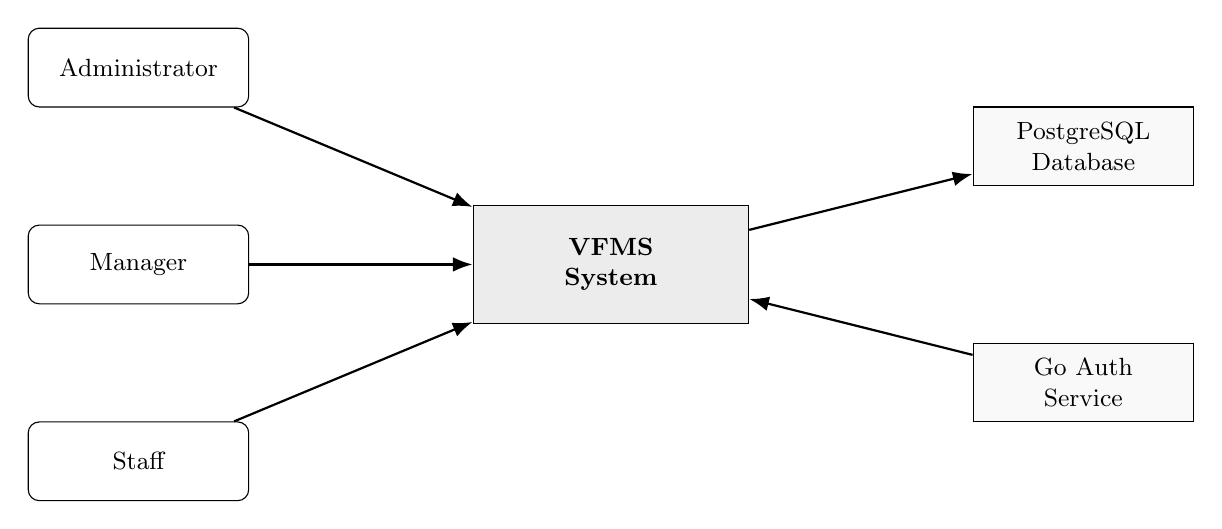
\begin{tikzpicture}[
    actor/.style={draw, rectangle, rounded corners, minimum width=2.8cm, minimum height=1cm, align=center, font=\small},
    sys/.style={draw, rectangle, minimum width=3.5cm, minimum height=1.5cm, align=center, font=\small\bfseries, fill=gray!15},
    ext/.style={draw, rectangle, minimum width=2.8cm, minimum height=1cm, align=center, font=\small, fill=gray!5},
    arrow/.style={-{Latex[length=2.5mm]}, thick}
]
    \node[sys] (vfms) at (0,0) {VFMS\\System};

    \node[actor] (admin) at (-6, 2.5) {Administrator};
    \node[actor] (mgr) at (-6, 0) {Manager};
    \node[actor] (staff) at (-6, -2.5) {Staff};

    \node[ext] (db) at (6, 1.5) {PostgreSQL\\Database};
    \node[ext] (auth) at (6, -1.5) {Go Auth\\Service};

    \draw[arrow] (admin) -- (vfms);
    \draw[arrow] (mgr) -- (vfms);
    \draw[arrow] (staff) -- (vfms);
    \draw[arrow] (vfms) -- (db);
    \draw[arrow] (auth) -- (vfms);
\end{tikzpicture}
\caption{System Context Diagram}
\label{fig:context}
\end{figure}

% ==================== 4. Architectural Design ====================
\section{Architectural Design}

\subsection{Chosen Architectural Style}
VFMS uses a \textbf{Three-Tier Layered Architecture} with a \textbf{microservices split} between the auth service and the fleet-data backend.

\begin{table}[H]
\centering
\begin{tabularx}{\textwidth}{|p{4cm}|X|}
\hline
\textbf{Field} & \textbf{Answer} \\
\hline
Architectural style & Three-Tier Layered Architecture + microservices split \\
\hline
Alternative considered & Monolithic single-tier application \\
\hline
Why this style was chosen & Splitting authentication into its own service means the backend database has no password column --- a compromise of the backend cannot leak credentials (NFR03). Layering separates UI, logic, and data access for easier testing and maintenance (NFR12). A monolith would couple everything together and blur the security boundary. \\
\hline
SRS requirements supported & NFR03, NFR04 (security), NFR12 (maintainability), FR01--FR02 (authentication and RBAC) \\
\hline
\end{tabularx}
\end{table}

\subsection{Architecture Diagram}

\begin{figure}[H]
\centering
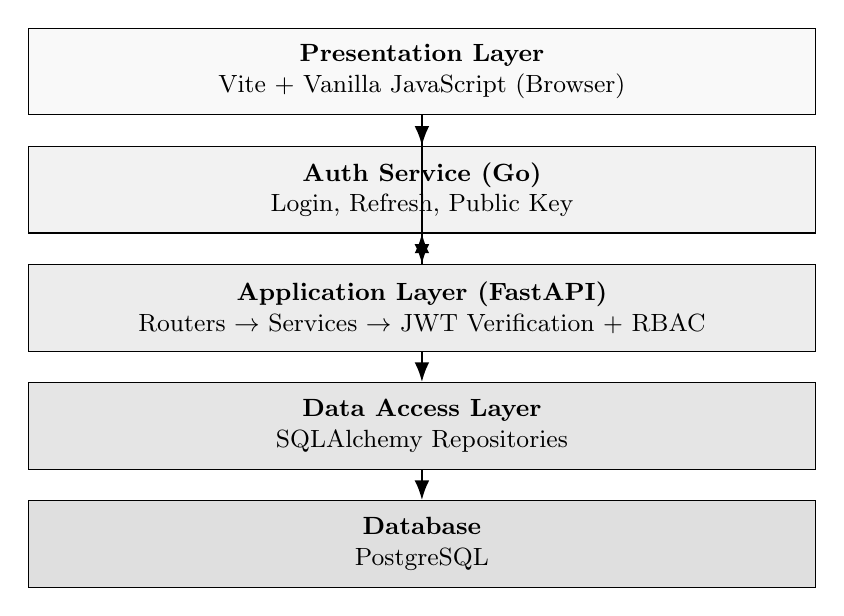
\begin{tikzpicture}[
    layer/.style={draw, rectangle, minimum width=10cm, minimum height=1.1cm, align=center, font=\small},
    arrow/.style={-{Latex[length=2.5mm]}, thick}
]
    \node[layer, fill=gray!5] (pres) at (0, 5) {\textbf{Presentation Layer}\\Vite + Vanilla JavaScript (Browser)};
    \node[layer, fill=gray!10] (auth) at (0, 3.5) {\textbf{Auth Service (Go)}\\Login, Refresh, Public Key};
    \node[layer, fill=gray!15] (app) at (0, 2) {\textbf{Application Layer (FastAPI)}\\Routers $\rightarrow$ Services $\rightarrow$ JWT Verification + RBAC};
    \node[layer, fill=gray!20] (data) at (0, 0.5) {\textbf{Data Access Layer}\\SQLAlchemy Repositories};
    \node[layer, fill=gray!25] (db) at (0, -1) {\textbf{Database}\\PostgreSQL};

    \draw[arrow] (pres) -- (auth);
    \draw[arrow] (pres) -- (app);
    \draw[arrow] (app) -- (auth);
    \draw[arrow] (app) -- (data);
    \draw[arrow] (data) -- (db);
\end{tikzpicture}
\caption{Layered Architecture of VFMS}
\label{fig:architecture}
\end{figure}

\subsection{Layer Descriptions}

\begin{table}[H]
\centering
\begin{tabularx}{\textwidth}{|p{3cm}|p{6cm}|p{4cm}|}
\hline
\textbf{Layer} & \textbf{Responsibility} & \textbf{Technology} \\
\hline
Presentation & Renders UI screens, handles user input, sends HTTP requests. Contains no business logic. & HTML5, CSS3, Vanilla JavaScript, Vite \\
\hline
Auth Service & Owns all credential handling. Hashes passwords, issues signed JWTs. Never sees fleet data. & Go 1.22 (standard library only) \\
\hline
Application & Business rules, RBAC checks, request validation. Verifies JWTs locally. & Python 3.11, FastAPI, Pydantic \\
\hline
Data Access & All database interactions through repositories. & SQLAlchemy ORM \\
\hline
Database & Persistent storage. Enforces referential integrity at schema level. & PostgreSQL 14 \\
\hline
\end{tabularx}
\end{table}

% ==================== 5. Class Design ====================
\section{Class Design}

\subsection{Class Diagram}

\begin{figure}[H]
\centering
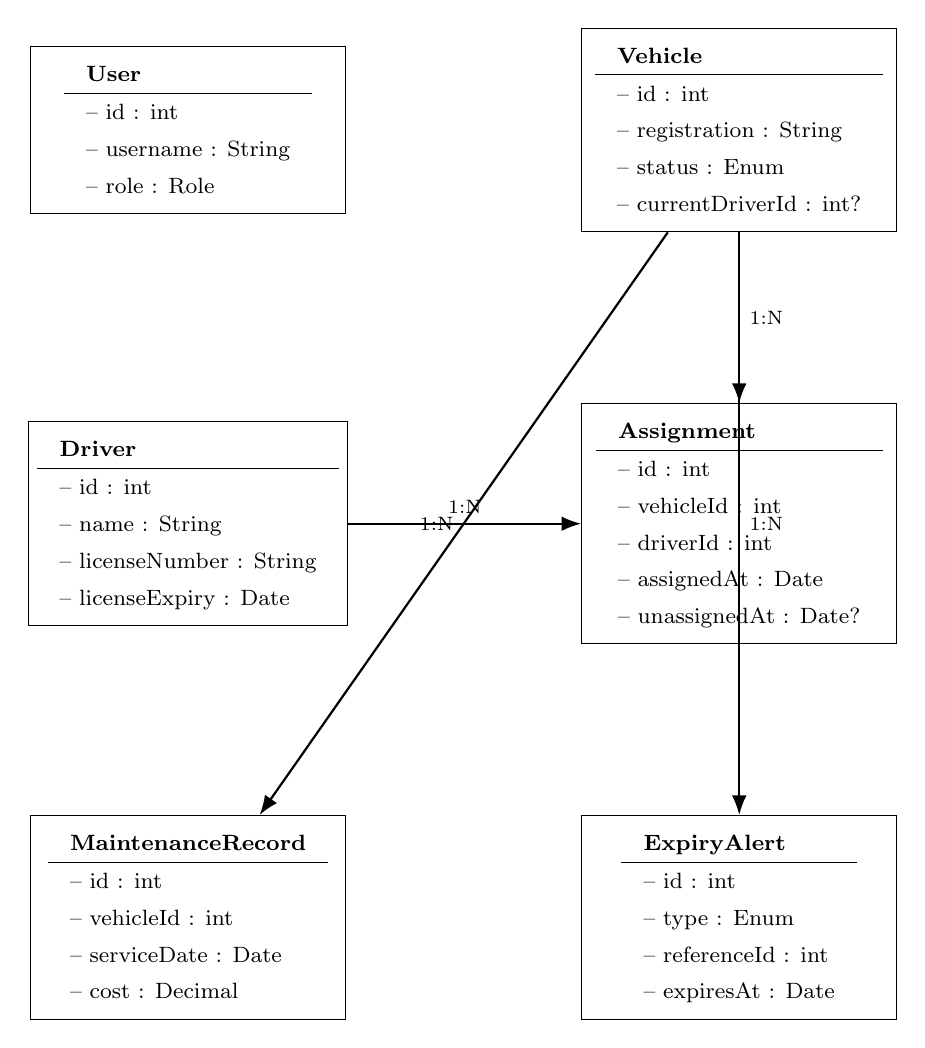
\begin{tikzpicture}[
    every node/.style={font=\footnotesize},
    arrow/.style={-{Latex[length=2.5mm]}, thick}
]

    % ---- User ----
    \node[draw, minimum width=4cm, minimum height=1.6cm] (user) at (0, 0) {
        \begin{tabular}{l}
        \textbf{User} \\ \hline
        -- id : int \\
        -- username : String \\
        -- role : Role \\
        \end{tabular}
    };

    % ---- Vehicle ----
    \node[draw, minimum width=4cm, minimum height=1.6cm] (veh) at (7, 0) {
        \begin{tabular}{l}
        \textbf{Vehicle} \\ \hline
        -- id : int \\
        -- registration : String \\
        -- status : Enum \\
        -- currentDriverId : int? \\
        \end{tabular}
    };

    % ---- Driver ----
    \node[draw, minimum width=4cm, minimum height=1.6cm] (drv) at (0, -5) {
        \begin{tabular}{l}
        \textbf{Driver} \\ \hline
        -- id : int \\
        -- name : String \\
        -- licenseNumber : String \\
        -- licenseExpiry : Date \\
        \end{tabular}
    };

    % ---- Assignment ----
    \node[draw, minimum width=4cm, minimum height=1.6cm] (asg) at (7, -5) {
        \begin{tabular}{l}
        \textbf{Assignment} \\ \hline
        -- id : int \\
        -- vehicleId : int \\
        -- driverId : int \\
        -- assignedAt : Date \\
        -- unassignedAt : Date? \\
        \end{tabular}
    };

    % ---- MaintenanceRecord ----
    \node[draw, minimum width=4cm, minimum height=1.6cm] (mnt) at (0, -10) {
        \begin{tabular}{l}
        \textbf{MaintenanceRecord} \\ \hline
        -- id : int \\
        -- vehicleId : int \\
        -- serviceDate : Date \\
        -- cost : Decimal \\
        \end{tabular}
    };

    % ---- ExpiryAlert ----
    \node[draw, minimum width=4cm, minimum height=1.6cm] (alert) at (7, -10) {
        \begin{tabular}{l}
        \textbf{ExpiryAlert} \\ \hline
        -- id : int \\
        -- type : Enum \\
        -- referenceId : int \\
        -- expiresAt : Date \\
        \end{tabular}
    };

    % ---- Relationships ----
    \draw[arrow] (veh) -- (asg) node[midway, right, font=\scriptsize] {1:N};
    \draw[arrow] (drv) -- (asg) node[midway, above, font=\scriptsize] {1:N};
    \draw[arrow] (veh) -- (mnt) node[midway, left, font=\scriptsize] {1:N};
    \draw[arrow] (veh) -- (alert) node[midway, right, font=\scriptsize] {1:N};

\end{tikzpicture}
\caption{UML Class Diagram}
\label{fig:class}
\end{figure}

\subsection{Class Descriptions}

\begin{table}[H]
\centering
\begin{tabularx}{\textwidth}{|p{2.5cm}|p{5cm}|p{3cm}|p{2cm}|}
\hline
\textbf{Class} & \textbf{Responsibility} & \textbf{Key Attributes} & \textbf{Related FR} \\
\hline
User & Represents an authenticated user. Managed by the auth service. & id, username, role & FR01, FR02, FR04 \\
\hline
Vehicle & Represents a fleet vehicle. Central entity for assignment and maintenance. & registration, status, currentDriverId & FR07--FR11, FR18--FR22 \\
\hline
Driver & Represents a licensed driver. Licence number is sensitive and role-restricted. & name, licenseNumber, licenseExpiry & FR12--FR17, FR27 \\
\hline
Assignment & Historical record of driver-vehicle assignments. Source of truth for history. & vehicleId, driverId, assignedAt, unassignedAt & FR18--FR22 \\
\hline
Maintenance & A single maintenance event for a vehicle. Used for cost reporting. & vehicleId, serviceDate, cost & FR23--FR26 \\
\hline
ExpiryAlert & Powers dashboard warnings for expiring documents. & type, referenceId, expiresAt & FR27--FR30 \\
\hline
\end{tabularx}
\end{table}

\subsection{Sequence Diagram --- User Login}

\begin{figure}[H]
\centering
\begin{tikzpicture}[
    lifeline/.style={draw, dashed, thick},
    head/.style={draw, rectangle, minimum width=2.5cm, minimum height=0.7cm, align=center, font=\footnotesize},
    arrow/.style={-{Latex[length=2.5mm]}, thick},
    return/.style={-{Latex[length=2.5mm]}, dashed, thick}
]
    \node[head] (u) at (0, 0) {Browser};
    \node[head] (a) at (4, 0) {Auth Service};
    \node[head] (b) at (8, 0) {Backend};
    \node[head] (d) at (12, 0) {Database};

    \draw[lifeline] (u) -- (0, -8);
    \draw[lifeline] (a) -- (4, -8);
    \draw[lifeline] (b) -- (8, -8);
    \draw[lifeline] (d) -- (12, -8);

    \draw[arrow] (0, -1.5) -- (4, -1.5) node[midway, above, font=\scriptsize] {1. POST /login};
    \draw[return] (4, -2.5) -- (0, -2.5) node[midway, above, font=\scriptsize] {2. JWT token};
    \draw[arrow] (0, -4) -- (8, -4) node[midway, above, font=\scriptsize] {3. GET /vehicles + Bearer JWT};
    \draw[arrow] (8, -5.5) -- (12, -5.5) node[midway, above, font=\scriptsize] {4. SQL query};
    \draw[return] (12, -7) -- (8, -7) node[midway, above, font=\scriptsize] {5. Rows};
\end{tikzpicture}
\caption{Sequence Diagram: Login and Fetch Vehicles}
\label{fig:sequence}
\end{figure}

% ==================== 6. Database Design ====================
\section{Database Design}

\subsection{Database Choice}

\begin{table}[H]
\centering
\begin{tabularx}{\textwidth}{|p{4cm}|X|}
\hline
\textbf{Field} & \textbf{Answer} \\
\hline
Database system & PostgreSQL 14 (MySQL 8.0 as alternative) \\
\hline
Type & Relational \\
\hline
Justification & Fleet data has clear relationships between vehicles, drivers, assignments, and maintenance. Foreign keys enforce integrity so records cannot be orphaned. Directly supports FR20 (prevent assignment of non-existent records). SQLite was rejected due to lack of multi-user concurrency. \\
\hline
\end{tabularx}
\end{table}

\subsection{Entity-Relationship Diagram}

\begin{figure}[H]
\centering
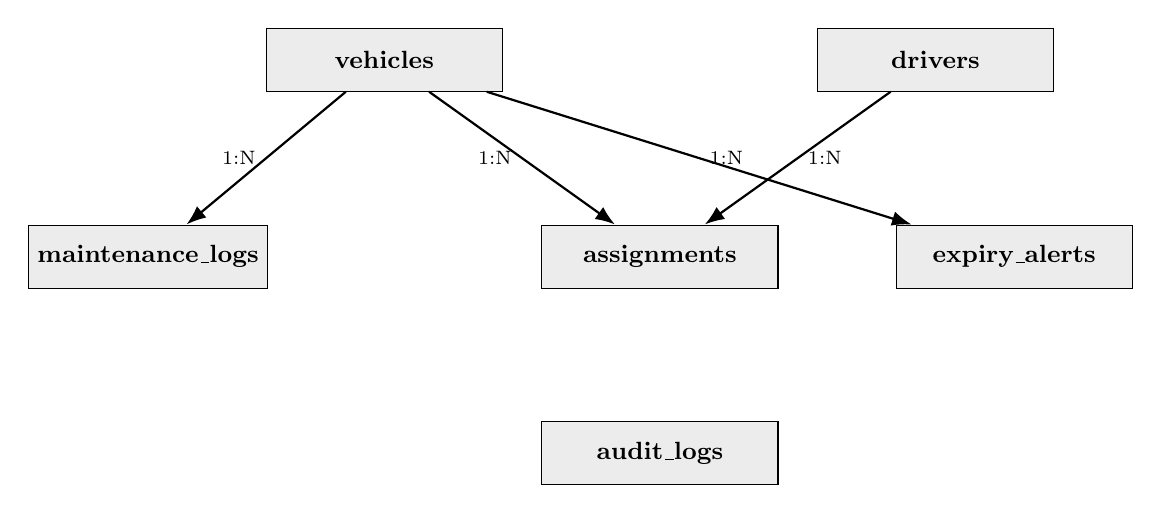
\begin{tikzpicture}[
    ent/.style={draw, rectangle, minimum width=3cm, minimum height=0.8cm, align=center, font=\small\bfseries, fill=gray!15},
    arrow/.style={-{Latex[length=2.5mm]}, thick}
]
    \node[ent] (veh) at (0, 4) {vehicles};
    \node[ent] (drv) at (7, 4) {drivers};
    \node[ent] (asg) at (3.5, 1.5) {assignments};
    \node[ent] (mnt) at (-3, 1.5) {maintenance\_logs};
    \node[ent] (exp) at (8, 1.5) {expiry\_alerts};
    \node[ent] (aud) at (3.5, -1) {audit\_logs};

    \draw[arrow] (veh) -- (asg) node[midway, left, font=\scriptsize] {1:N};
    \draw[arrow] (drv) -- (asg) node[midway, right, font=\scriptsize] {1:N};
    \draw[arrow] (veh) -- (mnt) node[midway, left, font=\scriptsize] {1:N};
    \draw[arrow] (veh) -- (exp) node[midway, right, font=\scriptsize] {1:N};
\end{tikzpicture}
\caption{Entity-Relationship Diagram}
\label{fig:erd}
\end{figure}

\subsection{Normalisation Rules Applied}

\begin{table}[H]
\centering
\begin{tabularx}{\textwidth}{|p{3.5cm}|p{5cm}|p{5cm}|}
\hline
\textbf{Rule} & \textbf{Meaning} & \textbf{How Applied} \\
\hline
One entity per table & Each table stores one type of thing & Separate tables for vehicles, drivers, assignments, maintenance, alerts \\
\hline
No repeated columns & Do not create item1, item2, item3 & Multiple services = multiple rows in maintenance\_logs, not columns \\
\hline
Use foreign keys & Store only the FK, not duplicated data & assignments stores vehicle\_id and driver\_id, not names or registration \\
\hline
\end{tabularx}
\end{table}

\subsection{Table Descriptions}

\begin{longtable}{|p{2.5cm}|p{3cm}|p{2cm}|p{2.5cm}|p{3.5cm}|}
\hline
\textbf{Table} & \textbf{Purpose} & \textbf{Primary Key} & \textbf{Foreign Keys} & \textbf{Key Attributes} \\
\hline
\endfirsthead
\hline
\textbf{Table} & \textbf{Purpose} & \textbf{Primary Key} & \textbf{Foreign Keys} & \textbf{Key Attributes} \\
\hline
\endhead
vehicles & One record per fleet vehicle & id & current\_driver\_id $\rightarrow$ drivers.id & registration\_number (unique), make, model, year, status, insurance\_expiry \\
\hline
drivers & One record per driver & id & none & first\_name, last\_name, license\_number (unique), license\_expiry, status \\
\hline
assignments & Driver-vehicle assignment history & id & vehicle\_id, driver\_id & assigned\_at, unassigned\_at, assigned\_by \\
\hline
maintenance & Every service event per vehicle & id & vehicle\_id & service\_date, cost, description, service\_provider \\
\hline
expiry\_alerts & Alerts for expiring documents & id & reference\_id & type, expires\_at, is\_triggered \\
\hline
audit\_logs & Record of all user actions & id & actor\_id & action, resource\_type, resource\_id, created\_at \\
\hline
\end{longtable}

% ==================== 7. Interface Design ====================
\section{Interface Design}

\subsection{Usability Principles Applied}

\begin{table}[H]
\centering
\begin{tabularx}{\textwidth}{|p{4cm}|X|}
\hline
\textbf{Principle} & \textbf{How Applied} \\
\hline
Visibility of system status & Loading spinner during search. Confirmation message after every save or delete. \\
\hline
Match with real world & Uses fleet terminology: ``Assign Driver'', ``Log Maintenance'', ``Expiring Soon''. \\
\hline
Error prevention & Registration and licence numbers checked for uniqueness before submit. Delete asks for confirmation. \\
\hline
Consistency and standards & Same button colours throughout: green for save, red for delete, blue for navigation. \\
\hline
Recognition over recall & Dashboard shows warning cards for expiring documents so users do not need to remember dates. \\
\hline
\end{tabularx}
\end{table}

\subsection{Screen Wireframes}

\subsubsection*{Screen 1 --- Login}

\begin{figure}[H]
\centering
\fbox{
\begin{minipage}{0.55\textwidth}
\centering
\vspace{0.3cm}
\textbf{VFMS Login}\\[0.5cm]
Username: \hrulefill \\[0.3cm]
Password: \hrulefill \\[0.5cm]
\fbox{Login}\\[0.3cm]
\textit{Error message area}\\
\vspace{0.3cm}
\end{minipage}
}
\caption{Login Screen}
\end{figure}

\subsubsection*{Screen 2 --- Dashboard}

\begin{figure}[H]
\centering
\fbox{
\begin{minipage}{0.85\textwidth}
\vspace{0.3cm}
\begin{tabular}{|p{2.5cm}|p{8cm}|}
\hline
\textbf{Menu} & \textbf{Dashboard --- Welcome} \\
\hline
Vehicles & Total: 25 \hspace{1cm} Active: 18 \hspace{1cm} In Maintenance: 4 \\
\hline
Drivers & \textbf{Expiry Warnings:} \\
\hline
Assignments & ! Driver licence expires in 5 days \\
\hline
Maintenance & ! Insurance expires in 20 days \\
\hline
Reports & ! Roadworthy expires in 28 days \\
\hline
 & [Add Vehicle] [Add Driver] [Log Maintenance] \\
\hline
\end{tabular}
\vspace{0.3cm}
\end{minipage}
}
\caption{Dashboard Screen}
\end{figure}

\subsubsection*{Screen 3 --- Add Vehicle}

\begin{figure}[H]
\centering
\fbox{
\begin{minipage}{0.6\textwidth}
\centering
\vspace{0.3cm}
\textbf{Add New Vehicle}\\[0.5cm]
\begin{tabular}{ll}
Registration*: & \hrulefill \\
Make*: & \hrulefill \\
Model*: & \hrulefill \\
Year*: & \hrulefill \\
Status*: & [Active] \\
\end{tabular}\\[0.5cm]
\fbox{Save} \hspace{0.5cm} \fbox{Cancel}\\[0.3cm]
\textit{* Required field}\\
\vspace{0.3cm}
\end{minipage}
}
\caption{Add Vehicle Screen}
\end{figure}

\subsection{Navigation Flow}

\begin{table}[H]
\centering
\begin{tabularx}{\textwidth}{|p{3cm}|p{2.5cm}|p{5cm}|p{3cm}|}
\hline
\textbf{Journey} & \textbf{Start} & \textbf{Steps} & \textbf{End} \\
\hline
Login & Login Screen & Enter credentials $\rightarrow$ Login $\rightarrow$ Redirect by role & Dashboard \\
\hline
Add vehicle & Dashboard & Click Add Vehicle $\rightarrow$ Fill form $\rightarrow$ Save & Vehicle List \\
\hline
Assign driver & Vehicle List & Click vehicle $\rightarrow$ Assign Driver $\rightarrow$ Select driver $\rightarrow$ Confirm & Vehicle Detail \\
\hline
Log maintenance & Dashboard & Click Log Maintenance $\rightarrow$ Fill form $\rightarrow$ Save & Maintenance History \\
\hline
\end{tabularx}
\end{table}

% ==================== 8. Design Traceability ====================
\section{Design Traceability Matrix}

\begin{longtable}{|p{1cm}|p{3.5cm}|p{5cm}|p{2cm}|p{2cm}|}
\hline
\textbf{Req ID} & \textbf{Requirement} & \textbf{Design Element} & \textbf{Section} & \textbf{Test} \\
\hline
\endfirsthead
\hline
\textbf{Req ID} & \textbf{Requirement} & \textbf{Design Element} & \textbf{Section} & \textbf{Test} \\
\hline
\endhead
FR01 & User login & User class, Login Screen, auth service & 4.2, 7.2 & UI test login form \\
\hline
FR02 & Role-based access control & require\_roles() dependency, RBAC map & 4.3, 5.2 & Unit test each role \\
\hline
FR03 & Restrict licence visibility & DriverPublicOut vs DriverOut schema & 5.2 & API test: staff cannot see licence \\
\hline
FR07 & Add vehicle & VehicleService.create(), Add Vehicle Screen & 5.2, 7.2 & UI test form submit \\
\hline
FR09 & Update vehicle & VehicleService.update(), PATCH endpoint & 5.2 & Unit test update \\
\hline
FR11 & Prevent duplicate registration & Unique constraint + 409 check & 6.4 & Integration test duplicate insert \\
\hline
FR17 & Show licence status & isLicenseValid() method, badge on list & 5.2, 7.2 & UI test badge states \\
\hline
FR18 & Assign driver to vehicle & VehicleService.assign\_driver(), assignments table & 5.2, 6.4 & Integration test assignment \\
\hline
FR21 & Prevent driver on two vehicles & Check currentDriverId is not null & 5.2 & Integration test expect 409 \\
\hline
FR23 & Log maintenance & MaintenanceRecord, POST /maintenance & 5.2, 7.2 & UI test log event \\
\hline
FR27 & Warn expiring licence & ExpiryAlert, dashboard warning card & 5.2, 7.2 & Integration test seed data \\
\hline
FR31 & Search vehicles & VehicleRepository.list(search=...) & 5.2, 6.4 & Performance test 500 rows \\
\hline
FR33 & Fleet summary report & GET /reports/summary, aggregate SQL & 5.2 & Integration test totals \\
\hline
NFR01 & Search under 3 seconds & Indexes on searchable fields & 6.4 & Performance test \\
\hline
NFR03 & Password security & PBKDF2 with 210,000 iterations & 4.3 & Unit test hash \\
\hline
NFR06 & Session timeout & Access token TTL 15 min + idle timer & 4.3 & Integration test idle \\
\hline
NFR13 & POPIA compliance & DriverPublicOut for staff, audit log & 4.3, 5.2 & Compliance checklist \\
\hline
\end{longtable}

% ==================== 9. Design Decisions ====================
\section{Design Decisions and Rationale}

\begin{longtable}{|p{2.5cm}|p{3.5cm}|p{2.5cm}|p{5cm}|}
\hline
\textbf{Decision} & \textbf{Options} & \textbf{Chosen} & \textbf{Rationale} \\
\hline
\endfirsthead
\hline
\textbf{Decision} & \textbf{Options} & \textbf{Chosen} & \textbf{Rationale} \\
\hline
\endhead
Architecture style & Monolith vs Layered + Microservices & Layered + Auth microservice & Backend has no password column, so a backend breach cannot leak credentials (NFR03). Layers are independently testable (NFR12). \\
\hline
Authentication & Sessions vs JWT vs OAuth & Username/password with RS256 JWT & JWT allows local verification (no round-trip per request). OAuth adds third-party dependencies. \\
\hline
Password hashing & SHA-256 vs bcrypt vs PBKDF2 & PBKDF2-HMAC-SHA256, 210k iterations & bcrypt unavailable in sandboxed build. PBKDF2 is NIST-recommended and works with Go standard library (zero dependencies). \\
\hline
Database & SQLite vs MySQL vs PostgreSQL & PostgreSQL (MySQL alternative) & Foreign keys with CASCADE needed for FR20. SQLite lacks multi-user concurrency. \\
\hline
Current driver pointer & Query history every time vs denormalised column & Denormalised currentDriverId + history table & Querying assignments on every read is slow. Denormalised pointer is a read optimisation. Both updates happen in one transaction to avoid drift. \\
\hline
Data visibility for staff & Filter on frontend vs two schemas on server & DriverPublicOut vs DriverOut & Frontend filtering can be bypassed by a direct API call. Server-side schema selection means the licence number is never sent (NFR04, POPIA). \\
\hline
Frontend framework & React vs Vue vs Vanilla JS & Vite + Vanilla JavaScript & Small number of pages. Team is more confident in plain JavaScript. No framework overhead. \\
\hline
\end{longtable}

% ==================== 10. AI Usage Declaration ====================
\section{AI Usage Declaration}

$\blacksquare$ AI tools were used. See below.

\begin{table}[H]
\centering
\begin{tabularx}{\textwidth}{|p{2.5cm}|p{3cm}|p{8cm}|}
\hline
\textbf{AI Tool} & \textbf{Sections} & \textbf{What was accepted / modified / rejected} \\
\hline
Claude (Anthropic) & Document structure and initial drafting  & \textbf{Accepted:} Template structure and standard definitions. \textbf{Modified:} All design elements reviewed . Class diagram tailored to real entities. NFR thresholds updated to specific values. \textbf{Rejected:} Generic classes not in the codebase (e.g. SMS Notification). Generic ``ReportManager'' class replaced with real /reports endpoints. \textbf{Added:} Denormalised currentDriverId decision was added by the team. \\
\hline
Claude (Anthropic) & Section 9 Design Decisions & \textbf{Accepted:} Table format. \textbf{Modified:} All rationale rewritten with actual project context  \textbf{Rejected:} Generic rationale like ``chosen for performance''. \\
\hline
\end{tabularx}
\end{table}


\vspace{1cm}

\begin{center}
\textbf{--- End of Software Design Document ---}\\[0.5cm]
\textbf{Version:} v1.0 \\
\textbf{Date:} 13/09/2026 \\
\textbf{Team 07 -- Vehicle Fleet Management System}
\end{center}

\end{document}